\subsection{Java Program}
The Java code is the backbone that interfaces between the separate modules of the host system. These modules are the Graphical User Inferface (GUI), the MATLAB\textsuperscript{\textregistered} optimisation, the MATLAB\textsuperscript{\textregistered} image processing and the profile server. Each module has a separate program class and thread. The result of the class interactions generates a desired sequence of velocity profiles to be enacted by the CNC machine. A thread is a term used to describe a linear process happening in parallel with multiple other processes. The general outlay of the components of the system can be seen in Figure\ref{fig:javaOverview}


\begin{figure}[htbp] 
\centering
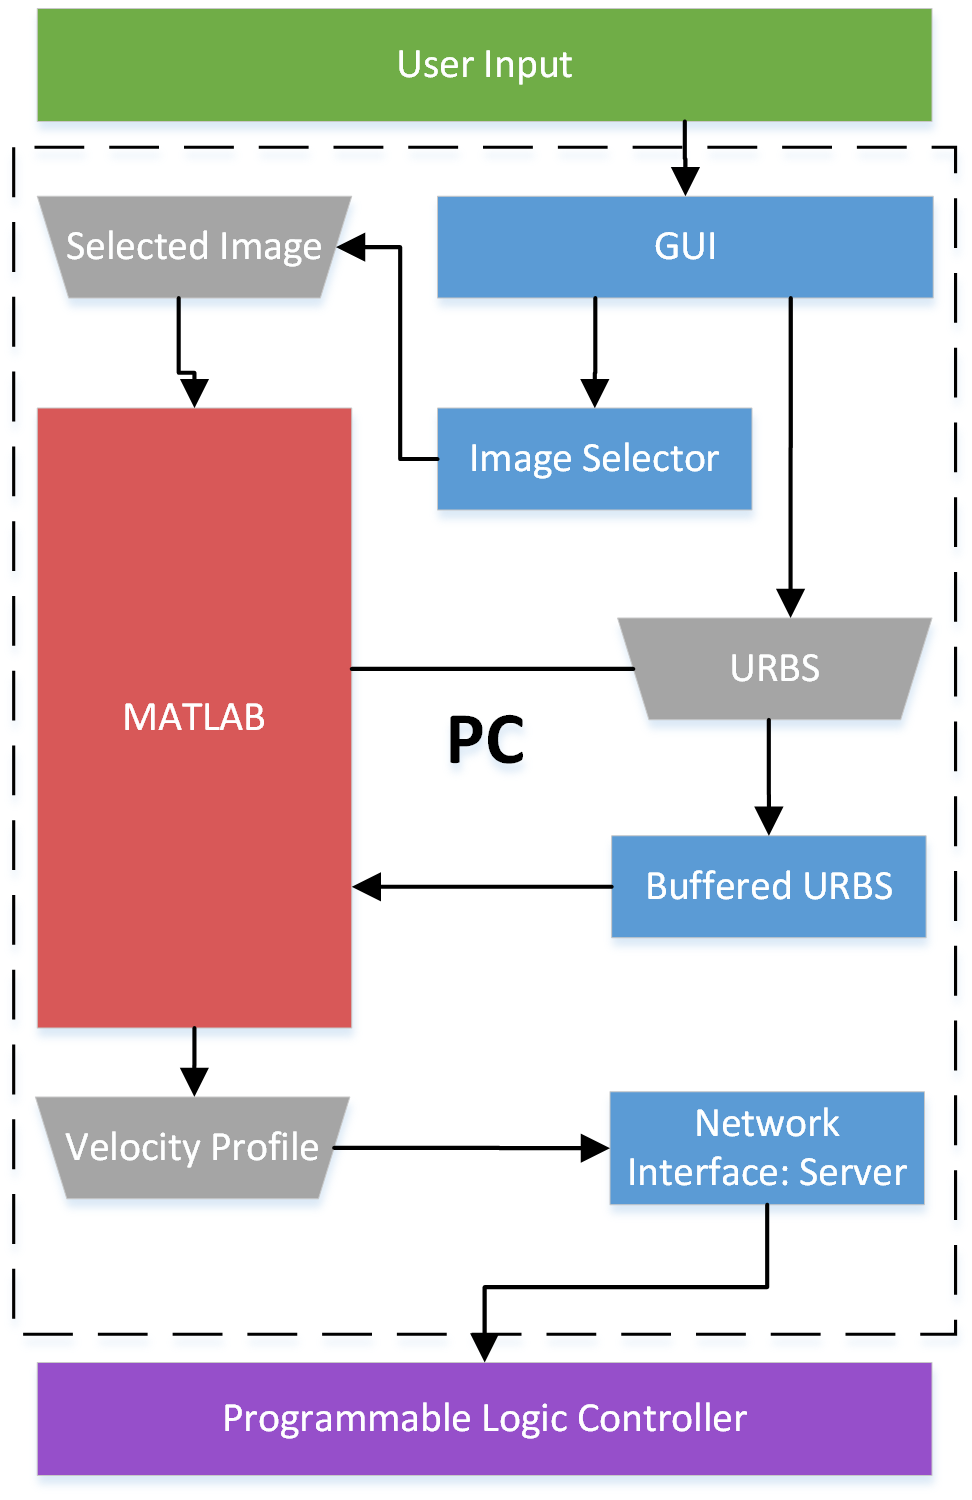
\includegraphics[width=0.6\textwidth]{figures/implementation/humanMachineInterface/systemDiagram2.png}
\caption[Human Machine Interface System Diagram]{This diagram demonstrates the interconnection of the components of the computer program that enables the user to interface with the DoodleBot. The components in BLUE represent Java modules. The component in RED represents the MATLAB\textsuperscript{\textregistered} interface.
\label{fig:javaOverview}}
\end{figure}

The overall system consists of separate program threads for each module. This allows processing operations to run in the background while the user can continue to interact with the program. User input occurs through the GUI program thread with direct input and input via selected images. The results are added to a buffer of curves which are displayed to the user. When the user is satisfied with the contents of the buffer they can order the program to print. This moves the buffered curves into a processing queue on the MATLAB\textsuperscript{\textregistered} interface program thread. This move means that the buffered curves will all be processed and printed. Curves are processed into velocity profiles with the optimisation algorithm in MATLAB\textsuperscript{\textregistered} and then loaded into the server program thread, which communicates the desired curves with the DoodleBot.